%------------------------------------------------------------
\title[01 - 初识计算机与程序设计]
{01 - 初识计算机与程序设计}

\subtitle{C++ 程序设计基础}

\author[Beiyu Li]
{Beiyu Li\\
\texttt{<sysulby@gmail.com>}}

% \institute[SOJ]
% {Sicily Online Judge}

\date[\today]
{\number\year 年 \number\month 月 \number\day 日}
%------------------------------------------------------------


\begin{document}

\author[sysulby]
{SOJ 信息学竞赛教练组}

\begin{frame}
    \titlepage
\end{frame}
\setcounter{framenumber}{0} % 标题页不编号


\section{计算机的组成}

%------------------------------------------------------------
\begin{frame}[fragile]
    \frametitle{你见过的计算机长什么样?}

    \begin{columns}
        \column{.5\textwidth}
        \begin{figure}
            
\includegraphics[width=.66\textwidth]{ch01/laptop.png}
        \end{figure}

        \column{.5\textwidth}
        \begin{figure}
            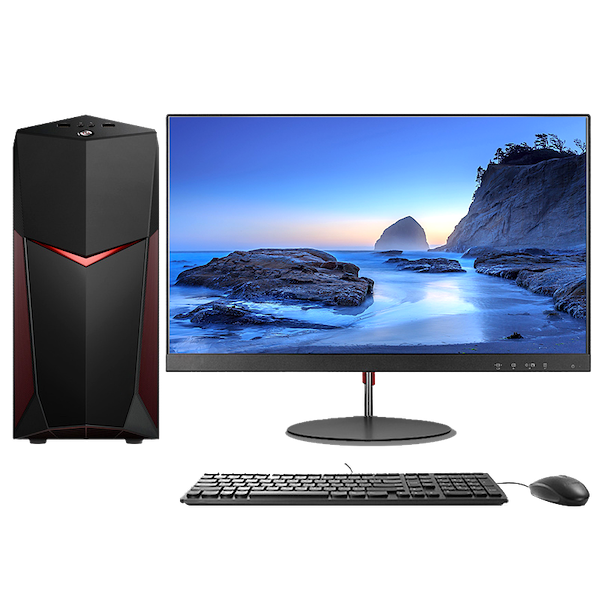
\includegraphics[width=.66\textwidth]{ch01/desktop.png}
        \end{figure}
    \end{columns}
    \begin{columns}
        \column{.33\textwidth}
        \begin{figure}
            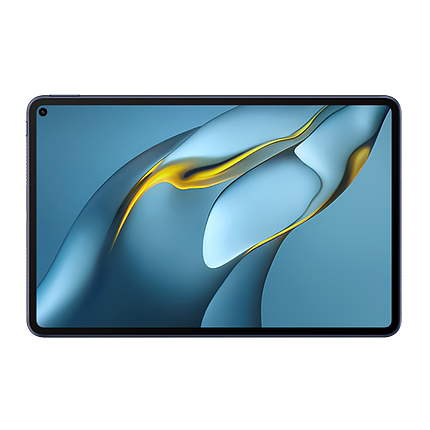
\includegraphics[width=.9\textwidth]{ch01/pad.png}
        \end{figure}

        \column{.33\textwidth}
        \begin{figure}
            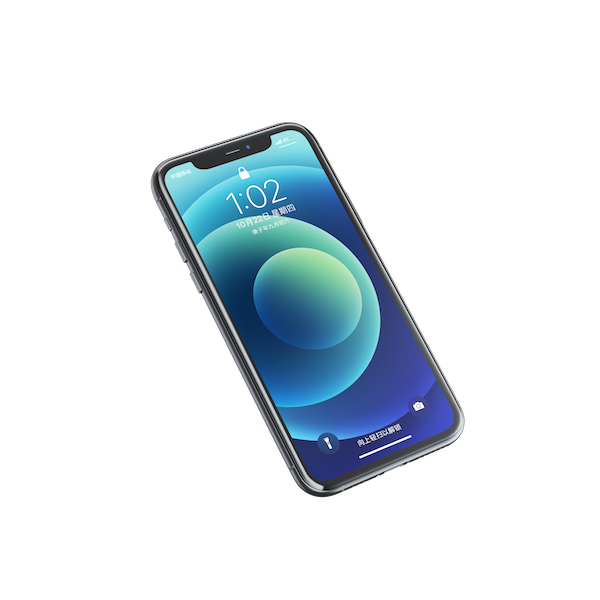
\includegraphics[width=.9\textwidth]{ch01/phone.png}
        \end{figure}

        \column{.34\textwidth}
        \begin{figure}
            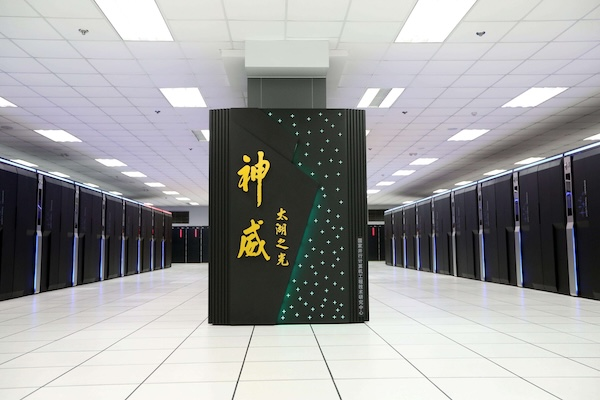
\includegraphics[width=.9\textwidth]{ch01/super.jpg}
        \end{figure}
    \end{columns}
\end{frame}
%------------------------------------------------------------

%------------------------------------------------------------
\begin{frame}[fragile]
    \frametitle{计算机由哪些部分组成?}

    \begin{overlayarea}{\textwidth}{\textheight}
        \begin{figure}
            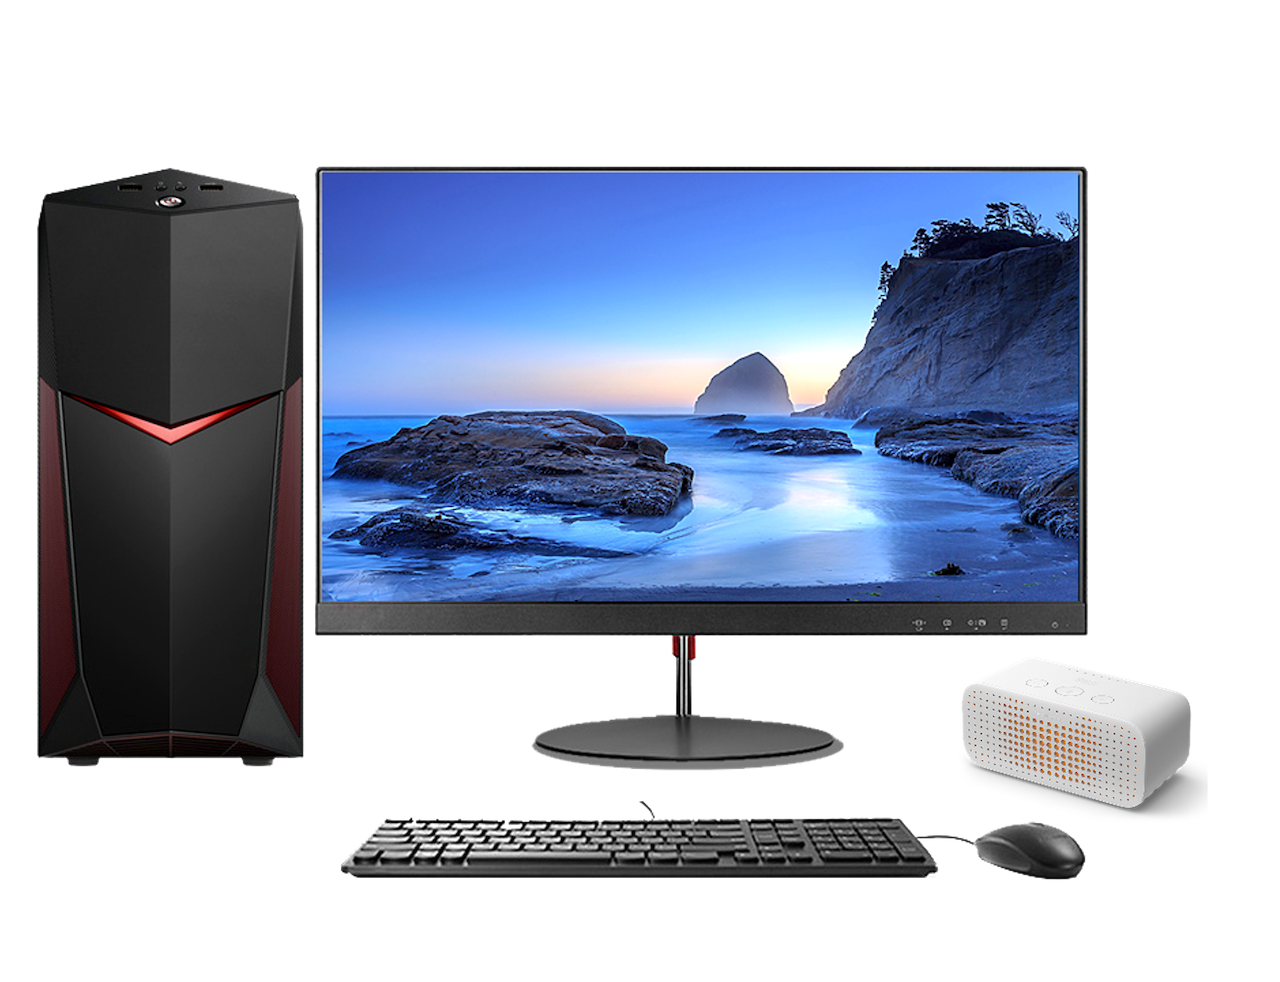
\includegraphics[width=.8\textwidth]{ch01/computer.png}
        \end{figure}

        \begin{textblock}{5}(3.5,3)
            \uncover<2->{
                主机
            }
        \end{textblock}

        \begin{textblock}{5}(7.5,3)
            \uncover<3->{
                显示器(输出设备)
            }
        \end{textblock}

        \begin{textblock}{5}(12,9)
            \uncover<4->{
                音箱(输出设备)
            }
        \end{textblock}

        \begin{textblock}{5}(11,12.5)
            \uncover<5->{
                鼠标(输入设备)
            }
        \end{textblock}

        \begin{textblock}{5}(5.5,12.5)
            \uncover<6->{
                键盘(输入设备)
            }
        \end{textblock}
    \end{overlayarea}
\end{frame}
%------------------------------------------------------------

%------------------------------------------------------------
\begin{frame}[fragile]
    \frametitle{主机里有什么?}

    \begin{overlayarea}{\textwidth}{\textheight}
        \begin{columns}
            \uncover<1->{
                \column{.33\textwidth}
                \begin{figure}
                    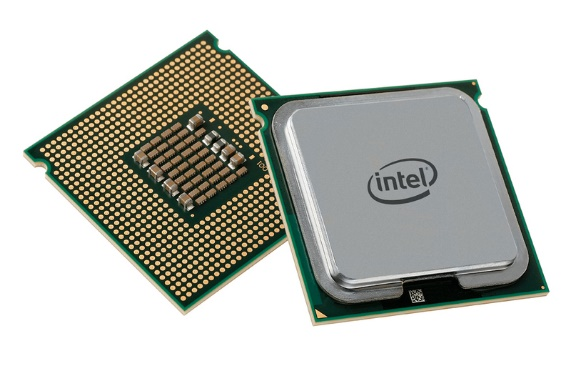
\includegraphics[width=.95\textwidth]{ch01/cpu.jpg}
                \end{figure}
            }

            \uncover<2->{
                \column{.33\textwidth}
                \begin{figure}
                    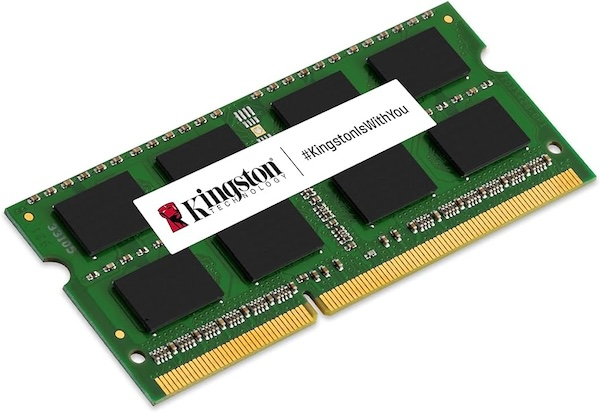
\includegraphics[width=.9\textwidth]{ch01/memory.jpg}
                \end{figure}
            }

            \uncover<3->{
                \column{.34\textwidth}
                \begin{figure}
                    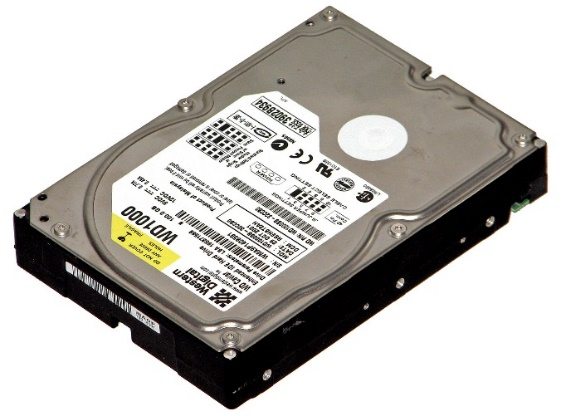
\includegraphics[width=.9\textwidth]{ch01/disk.jpg}
                \end{figure}
            }
        \end{columns}
        \begin{columns}
            \uncover<4->{
                \column{.4\textwidth}
                \begin{figure}
                    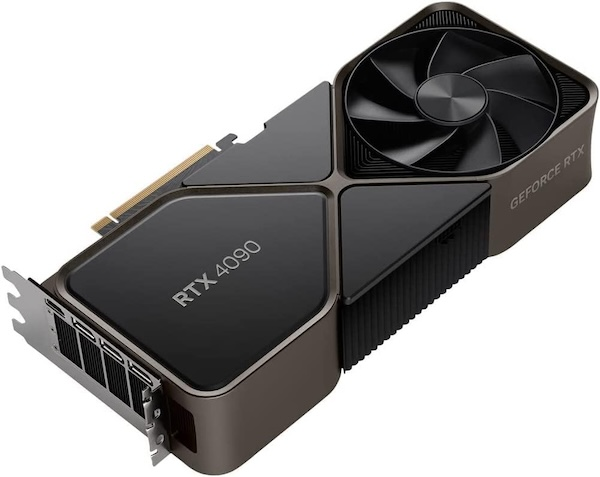
\includegraphics[width=.8\textwidth]{ch01/gpu.jpg}
                \end{figure}
            }

            \uncover<5->{
                \column{.6\textwidth}
                \begin{figure}
                    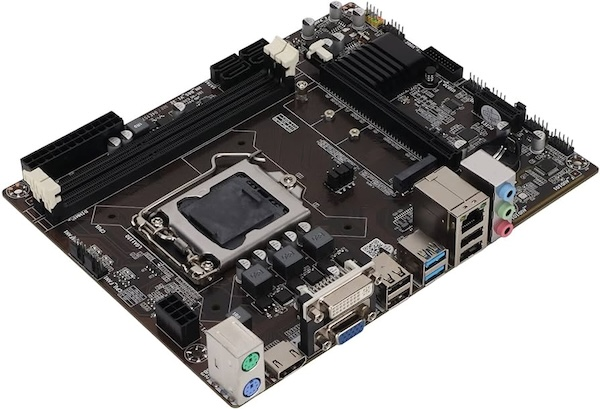
\includegraphics[width=.8\textwidth]{ch01/motherboard.jpg}
                \end{figure}
            }
        \end{columns}
    \end{overlayarea}
\end{frame}
%------------------------------------------------------------

%------------------------------------------------------------
\begin{frame}[fragile]
    \frametitle{计算机的组成部件}

    \begin{itemize}[<+->]
        \item 输入设备:键盘、鼠标、触摸屏等
        \item 输出设备:显示器、打印机、音箱等
        \item 中央处理器(即 CPU),含有运算器和控制器
        \item 存储器:内存、硬盘等
        \item 其他设备(可选):独立显卡、网卡等
    \end{itemize}
\end{frame}
%------------------------------------------------------------

%------------------------------------------------------------
\begin{frame}[fragile]
    \frametitle{讨论}

    \begin{block}{}
        \vspace{.5cm}
        \begin{center}
            {\Large 你用计算机做过什么事情?}
        \end{center}
        \vspace{.5cm}
    \end{block}
\end{frame}
%------------------------------------------------------------

\subsection{计算机的工作原理}

%------------------------------------------------------------
\begin{frame}[fragile]
    \frametitle{计算机如何工作}

    \begin{figure}
        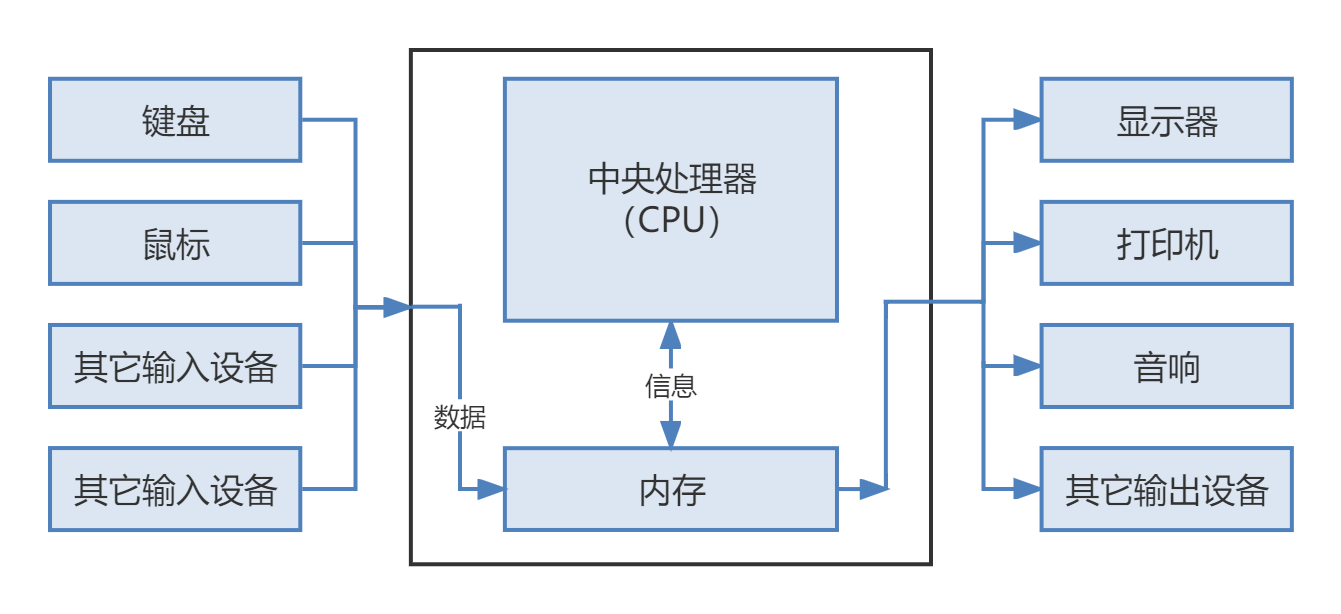
\includegraphics[width=.9\textwidth]{ch01/system.png}
    \end{figure}

    \begin{overlayarea}{\textwidth}{.2\textheight}
        \only<2> {程序从输入设备中获得用户的输入信息,然后对信息进行处理,再把处理结果通过输出设备展示给用户。}
        \only<3> {处理过程是 CPU 和内存一起完成的:CPU 执行“处理动作”,而内存中既存放了用户输入数据,也存放了告诉 CPU 如何处理数据的“说明书”——程序。}
        \only<4> {计算机之所以可以完成不同的功能,正是因为我们给它编写了不同的程序。}
    \end{overlayarea}
\end{frame}
%------------------------------------------------------------


\section{程序设计及编程语言的发展}

%------------------------------------------------------------
\begin{frame}[fragile]
    \frametitle{什么是程序}

    \begin{itemize}[<+->]
        \item 程序是给计算机的指令,我们通过程序告诉计算机做什么和怎么做
        \item 计算机不懂得人类的语言(自然语言),所以你需要用计算机语言(编程语言)来和计算机交流
        \item 因此,程序需要使用编程语言来编写
    \end{itemize}
\end{frame}
%------------------------------------------------------------

%------------------------------------------------------------
\begin{frame}[fragile]
    \frametitle{程序设计语言的发展}

    \begin{itemize}
        \item<1-> 机器语言(Machine Language)\hfill \textcolor{red}{\lstinline|110110101001101|}

            \begin{itemize}
                \item 机器语言是每台计算机的 CPU 指令集合
            \end{itemize}

        \item<2-> 汇编语言(Assembly Language)\hfill \textcolor{red}{\lstinline|ADD R1, R2, R3|}

            \begin{itemize}
                \item 汇编语言用符号(助记符)来代替 0/1 码,运行时通过汇编器转换为机器语言
            \end{itemize}

        \item<3-> 高级语言(High-level Languages)\hfill \textcolor{red}{\lstinline|C = A + B|}

            \begin{itemize}
                \item 高级语言用自然语言符号来代替 0/1 码,运行时通过编译器转换为机器语言
                \item 高级语言更接近我们日常使用的自然语言
            \end{itemize}

    \end{itemize}
\end{frame}
%------------------------------------------------------------

%------------------------------------------------------------
\begin{frame}[fragile]
    \frametitle{C++ 语言的特点}

    \begin{itemize}
        \item<1-> C/C++ 的应用范围广

            \begin{itemize}
                \item 许多设备的驱动程序和操作系统的都是用 C/C++ 写的
                \item 编程开发方面的工作中 C/C++ 仍然是热门语言
            \end{itemize}

        \item<2-> C/C++ 的程序运行效率更快

        \item<3-> C/C++ 是高级语言中最接近低级语言的,因而如果想更深入了解计算机是如何运作的,C/C++ 是首选

        \item<4-> 熟练掌握 C/C++ 语言,在学习其他高级编程语言时更加轻松
    \end{itemize}
\end{frame}
%------------------------------------------------------------

%------------------------------------------------------------
\begin{frame}[fragile]
    \frametitle{C++ 编译运行的流程}

    \begin{figure}
        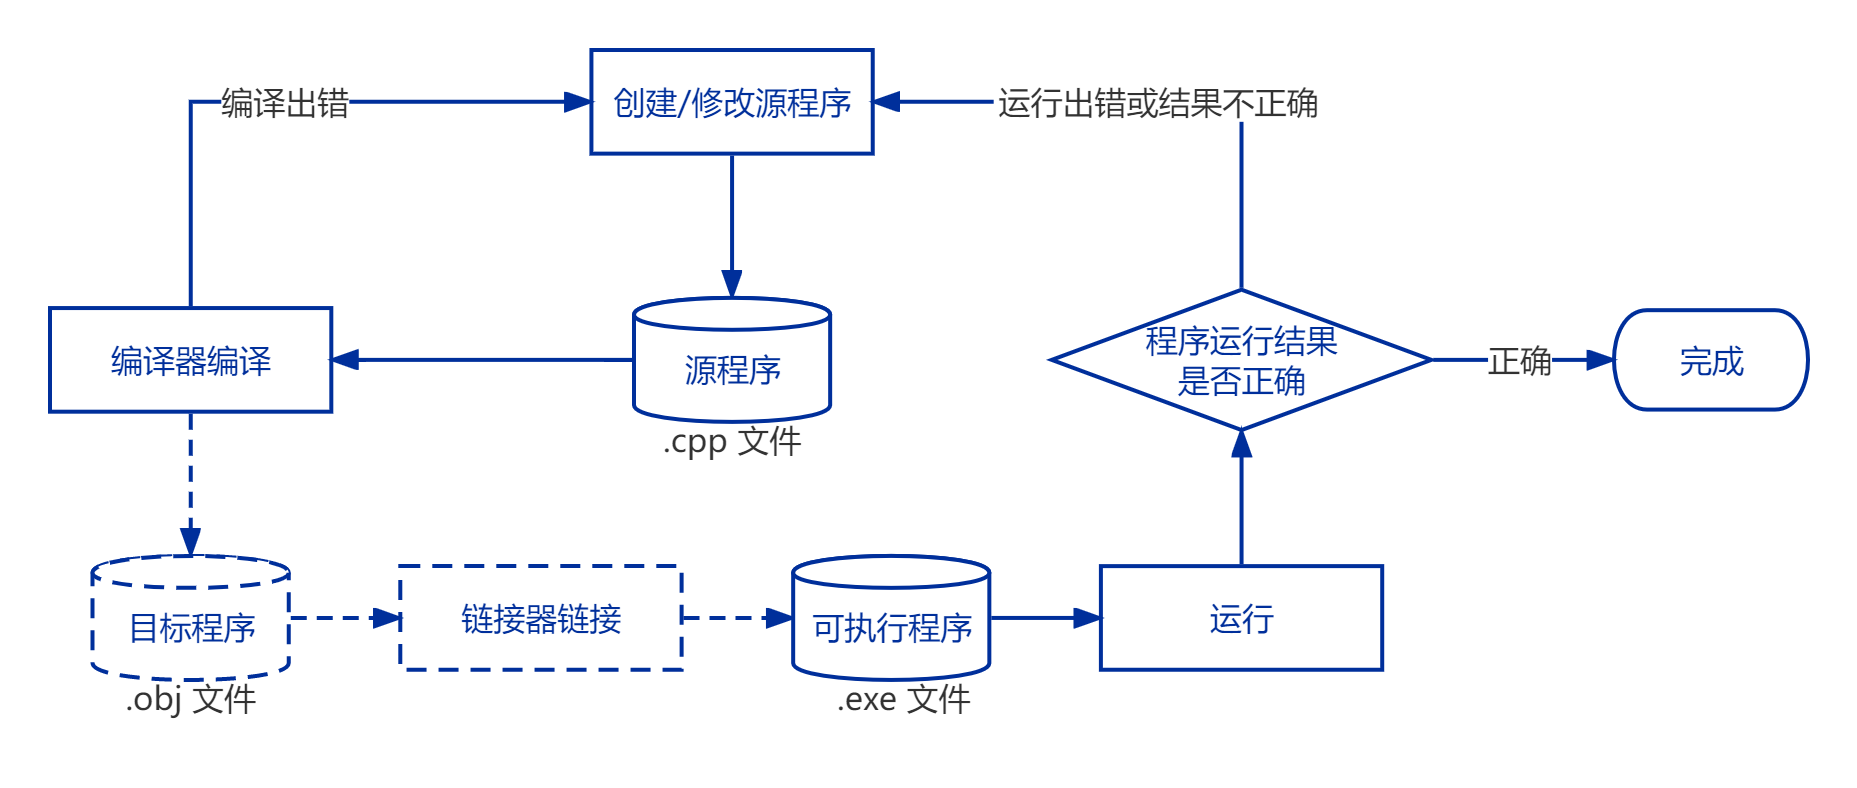
\includegraphics[width=\textwidth]{ch01/compiler.png}
    \end{figure}
\end{frame}
%------------------------------------------------------------


\section{编写第一个程序}

%------------------------------------------------------------
\begin{frame}[fragile]
    \frametitle{IDE 的使用}

    \begin{figure}
        \only<1>{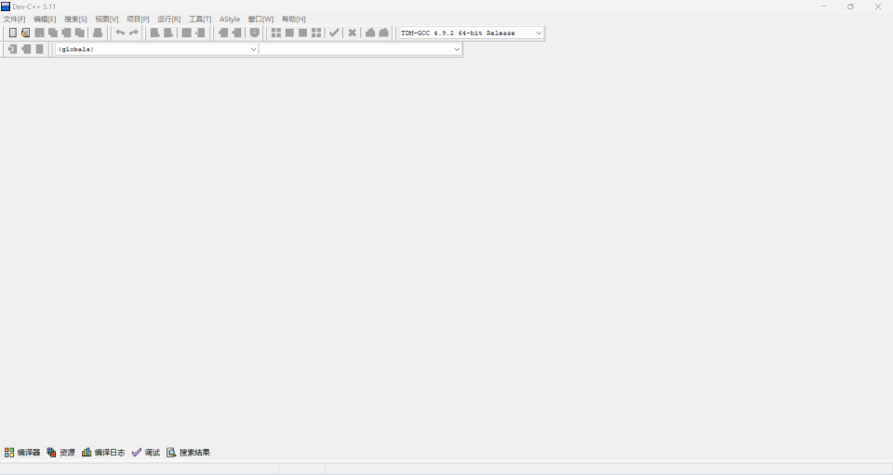
\includegraphics[width=\textwidth]{ch01/ide_1.png}}
        \only<2>{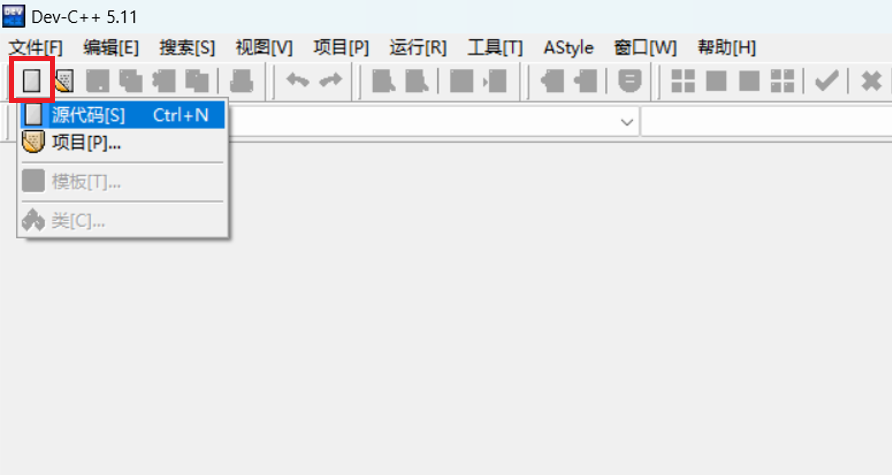
\includegraphics[width=\textwidth]{ch01/ide_2.png}}
        \only<3>{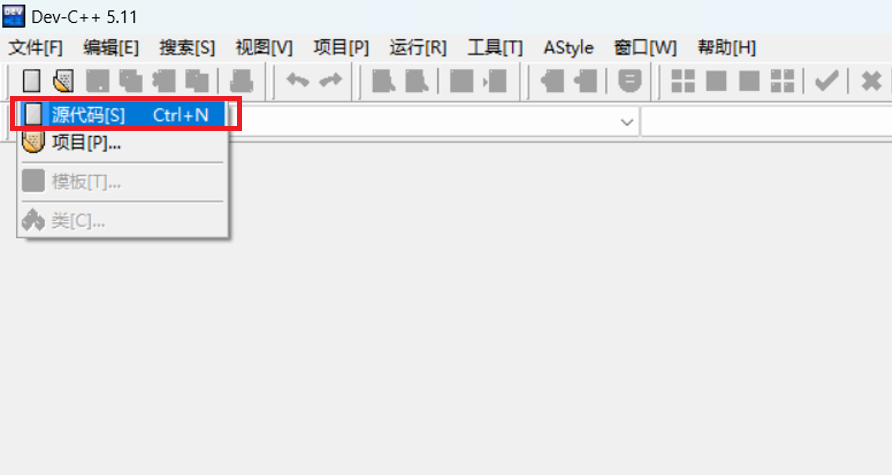
\includegraphics[width=\textwidth]{ch01/ide_3.png}}
        \only<4>{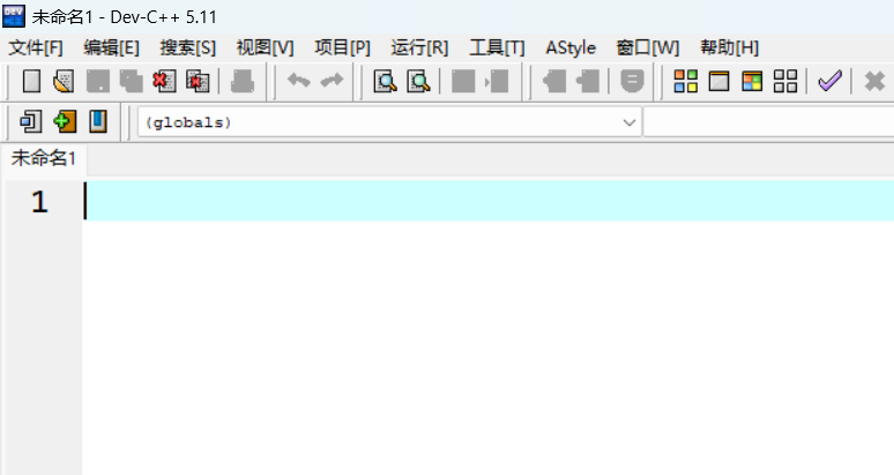
\includegraphics[width=\textwidth]{ch01/ide_new_code.png}}
        \only<5>{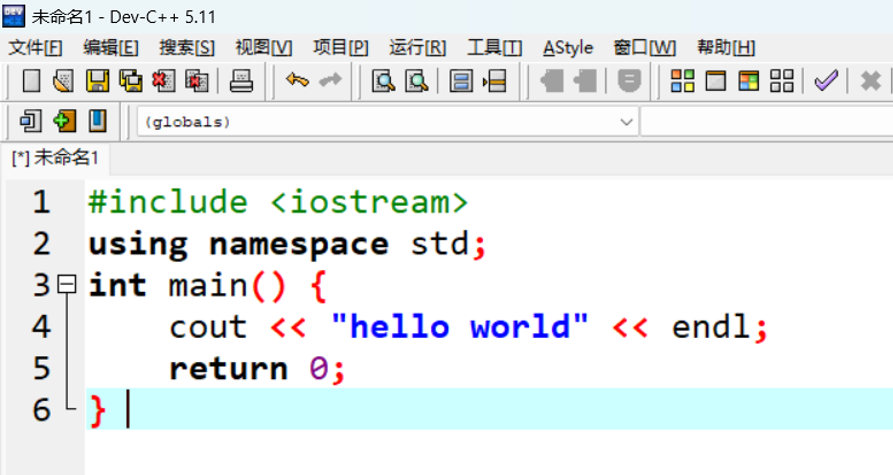
\includegraphics[width=\textwidth]{ch01/ide_code.png}}
        \only<6>{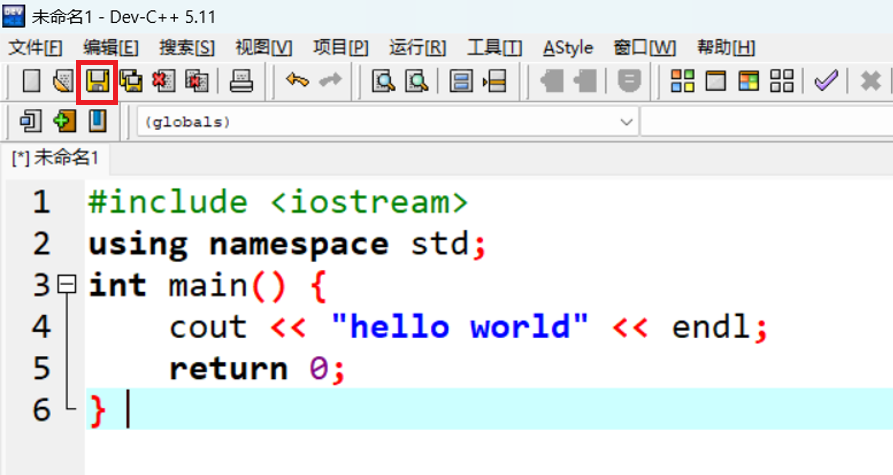
\includegraphics[width=\textwidth]{ch01/code_saving.png}}
        \only<7>{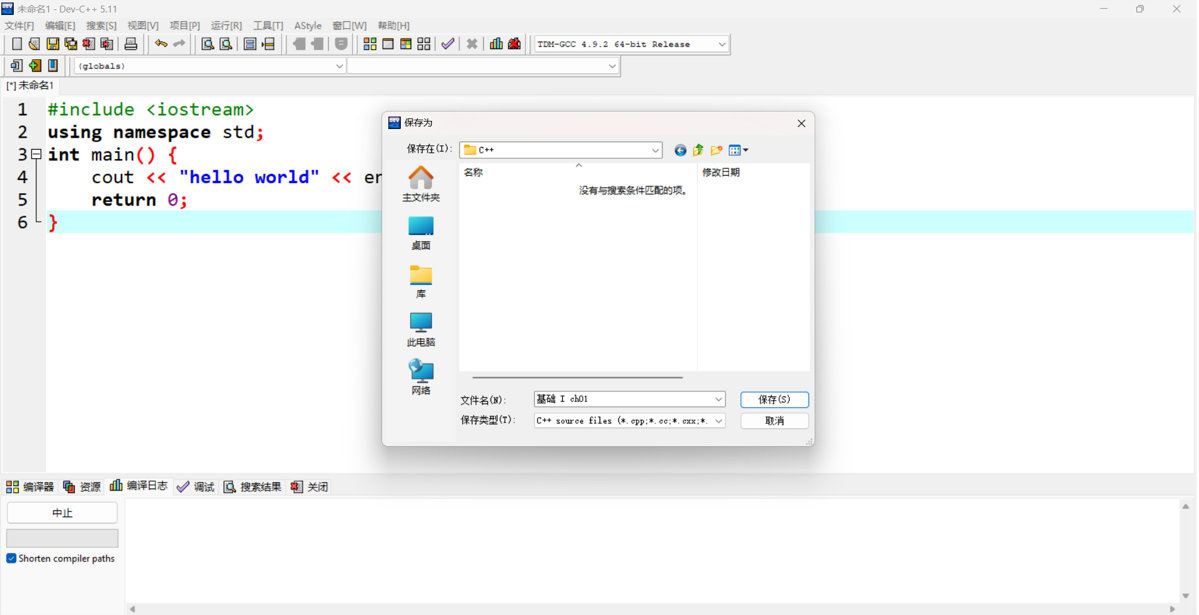
\includegraphics[width=\textwidth]{ch01/ide_code_save.png}}
        \only<8>{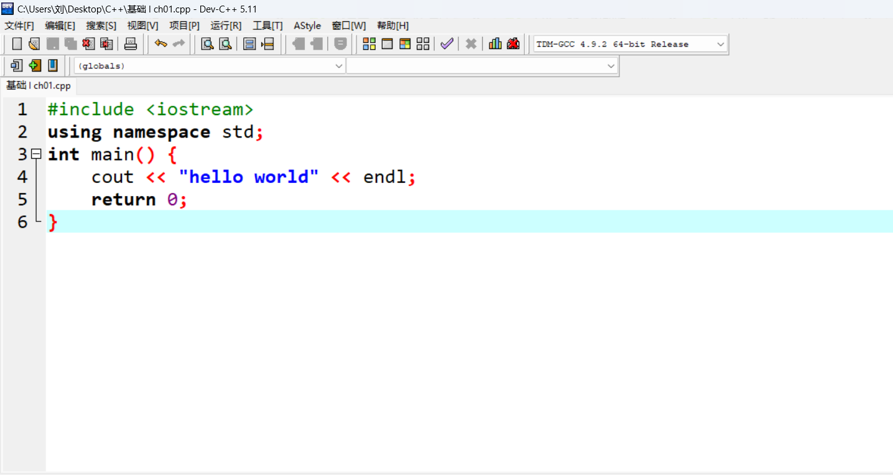
\includegraphics[width=\textwidth]{ch01/ide_code_saved.png}}
        \only<9>{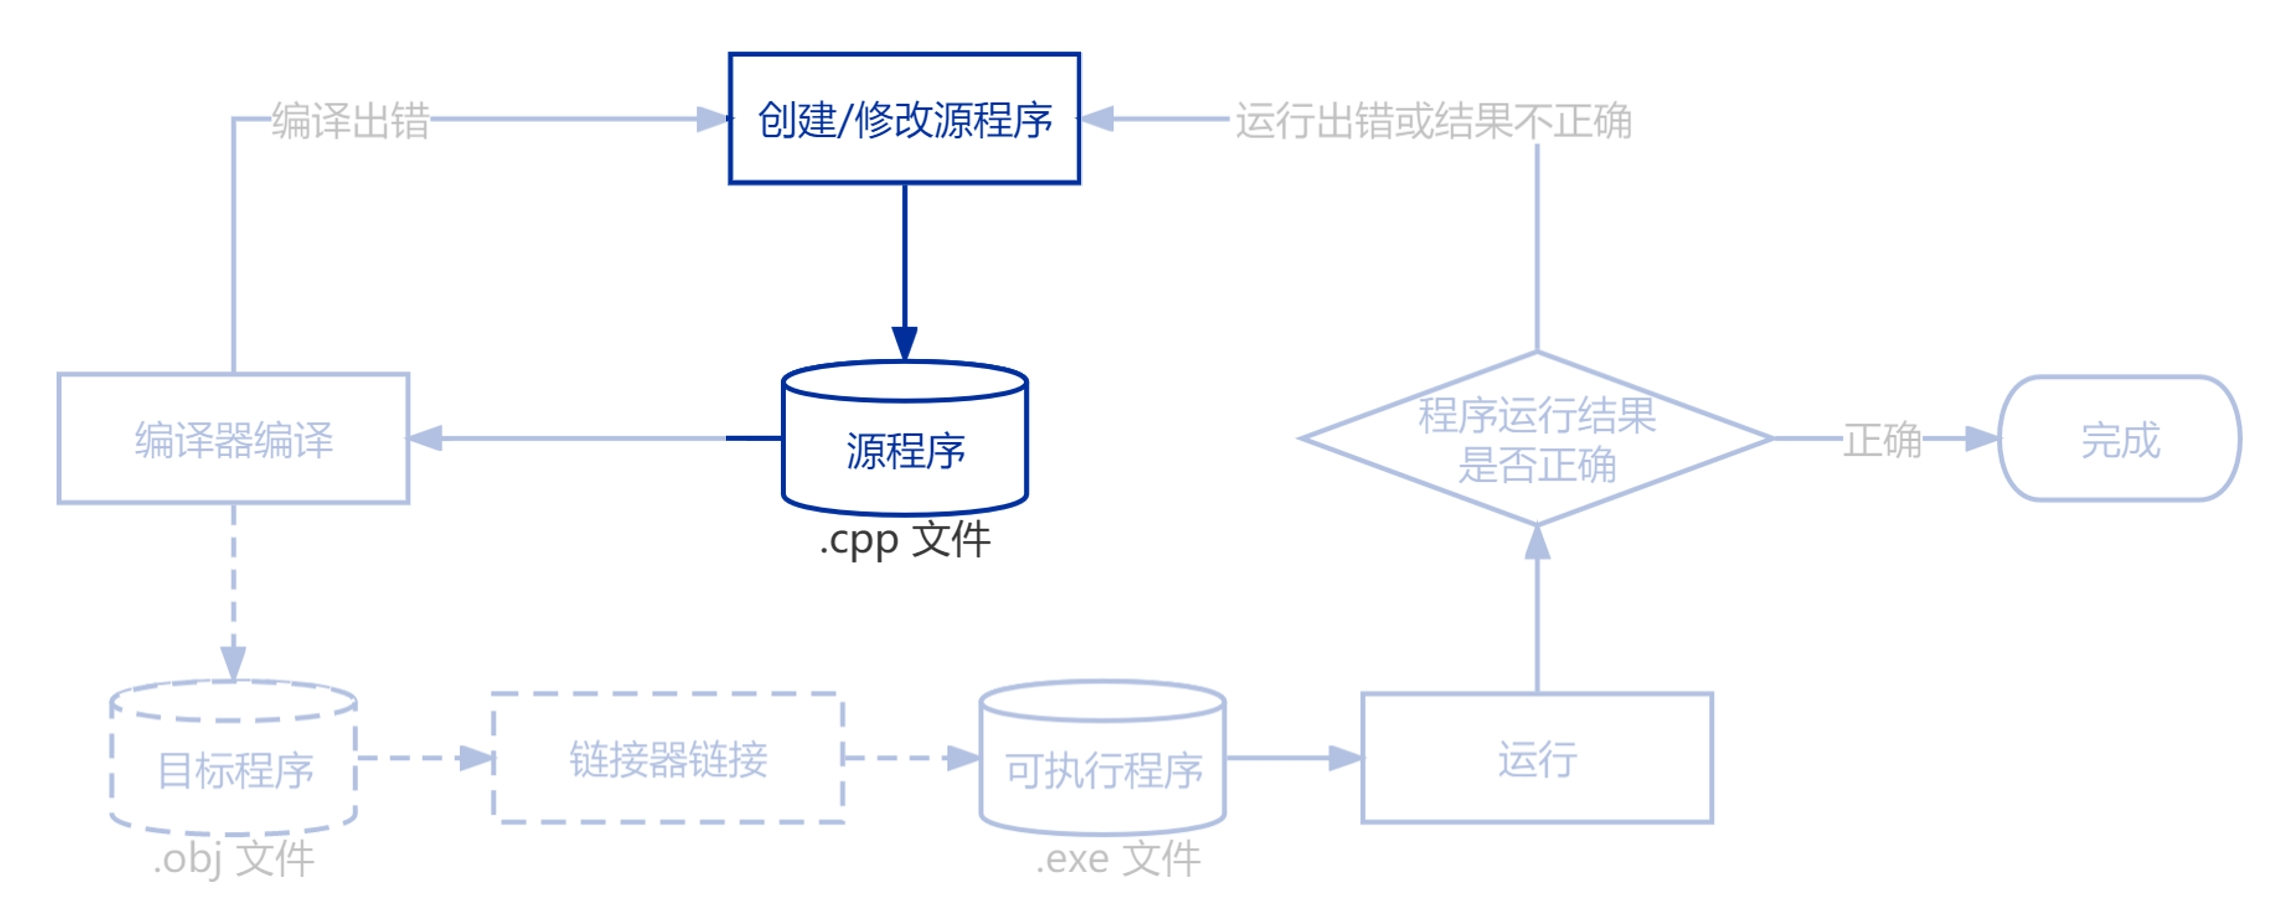
\includegraphics[width=\textwidth]{ch01/create_file.png}}
        \only<10>{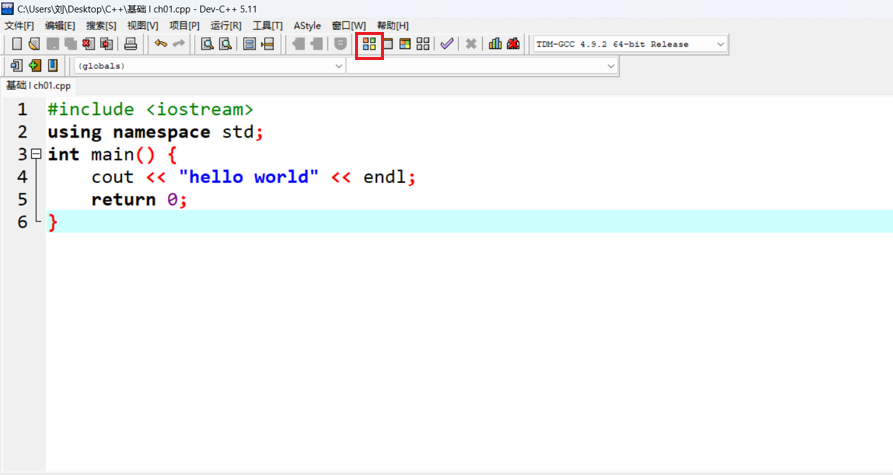
\includegraphics[width=\textwidth]{ch01/code_compile.png}}
        \only<11>{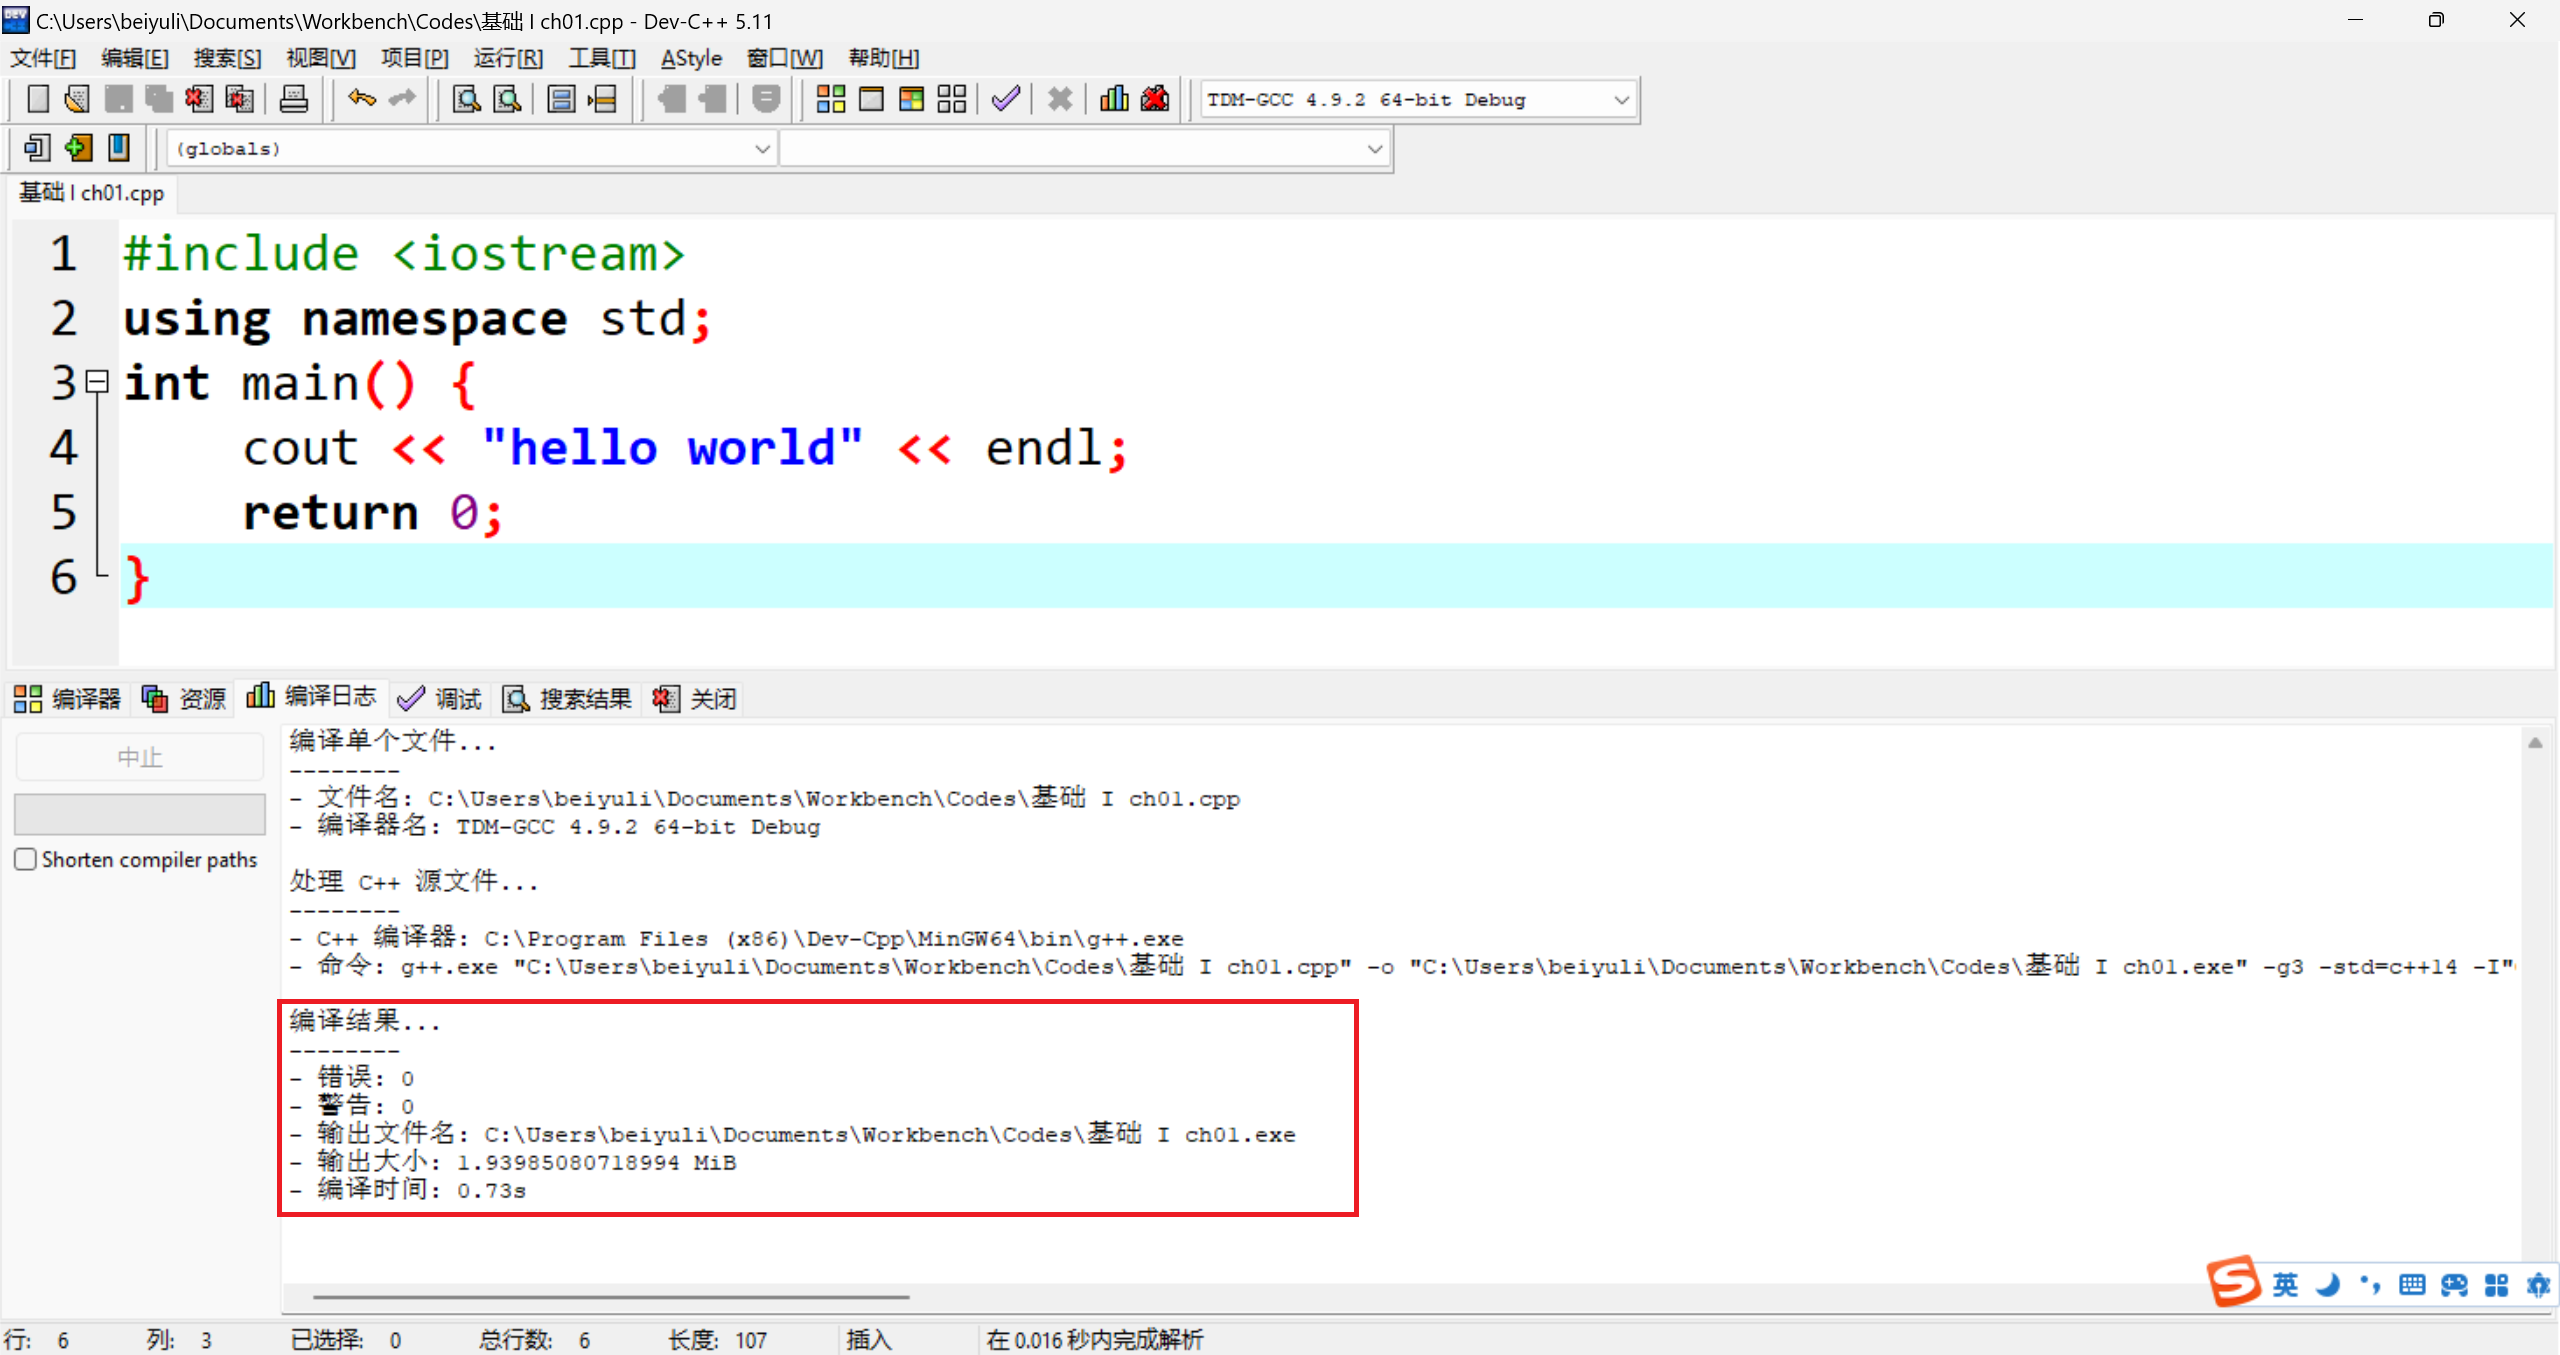
\includegraphics[width=\textwidth]{ch01/code_compiled.png}}
        \only<12>{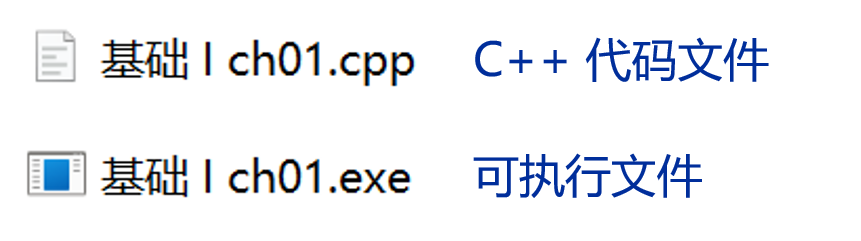
\includegraphics[width=\textwidth]{ch01/ide_code_fileRoute.png}}
        \only<13>{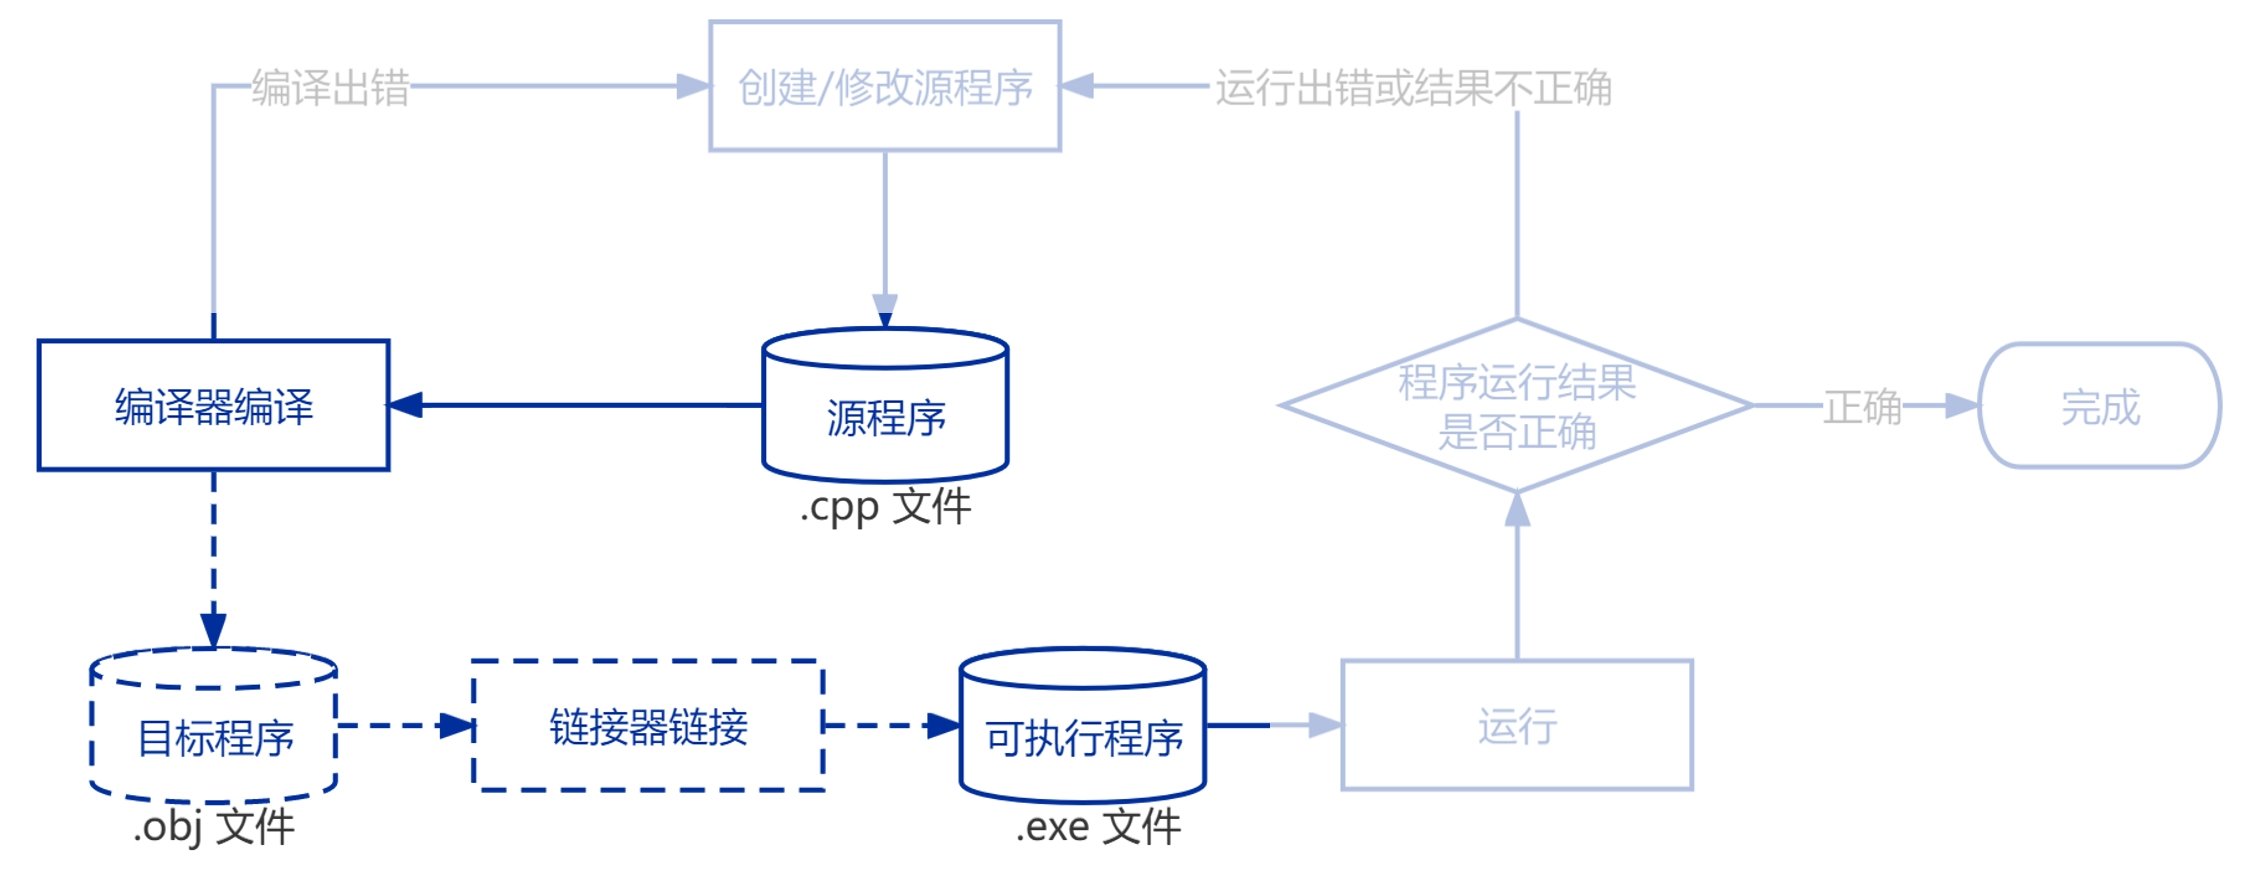
\includegraphics[width=\textwidth]{ch01/compile.png}}
        \only<14>{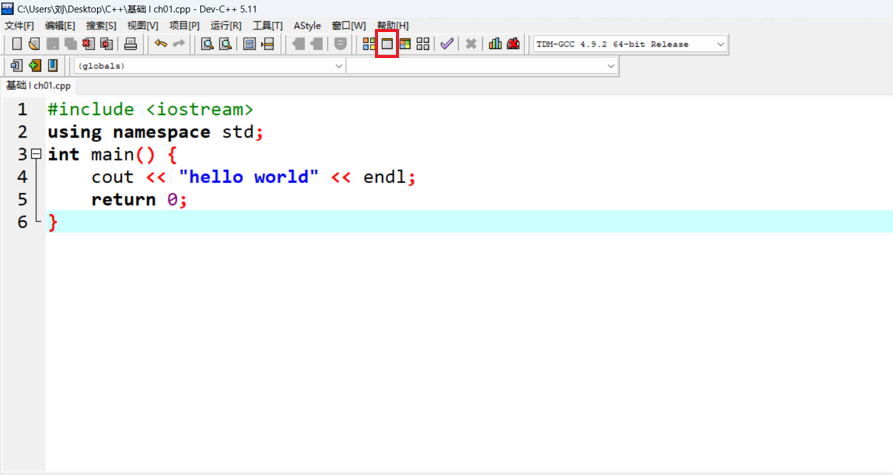
\includegraphics[width=\textwidth]{ch01/code_run.png}}
        \only<15>{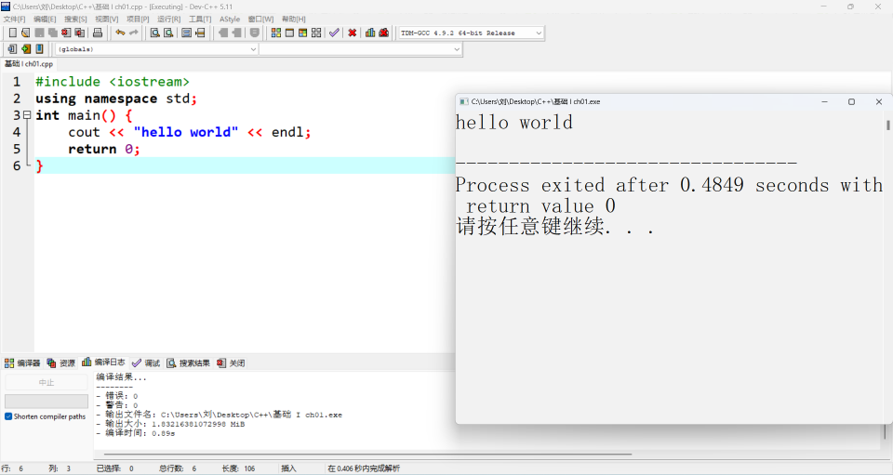
\includegraphics[width=\textwidth]{ch01/ide_run.png}}
        \only<16>{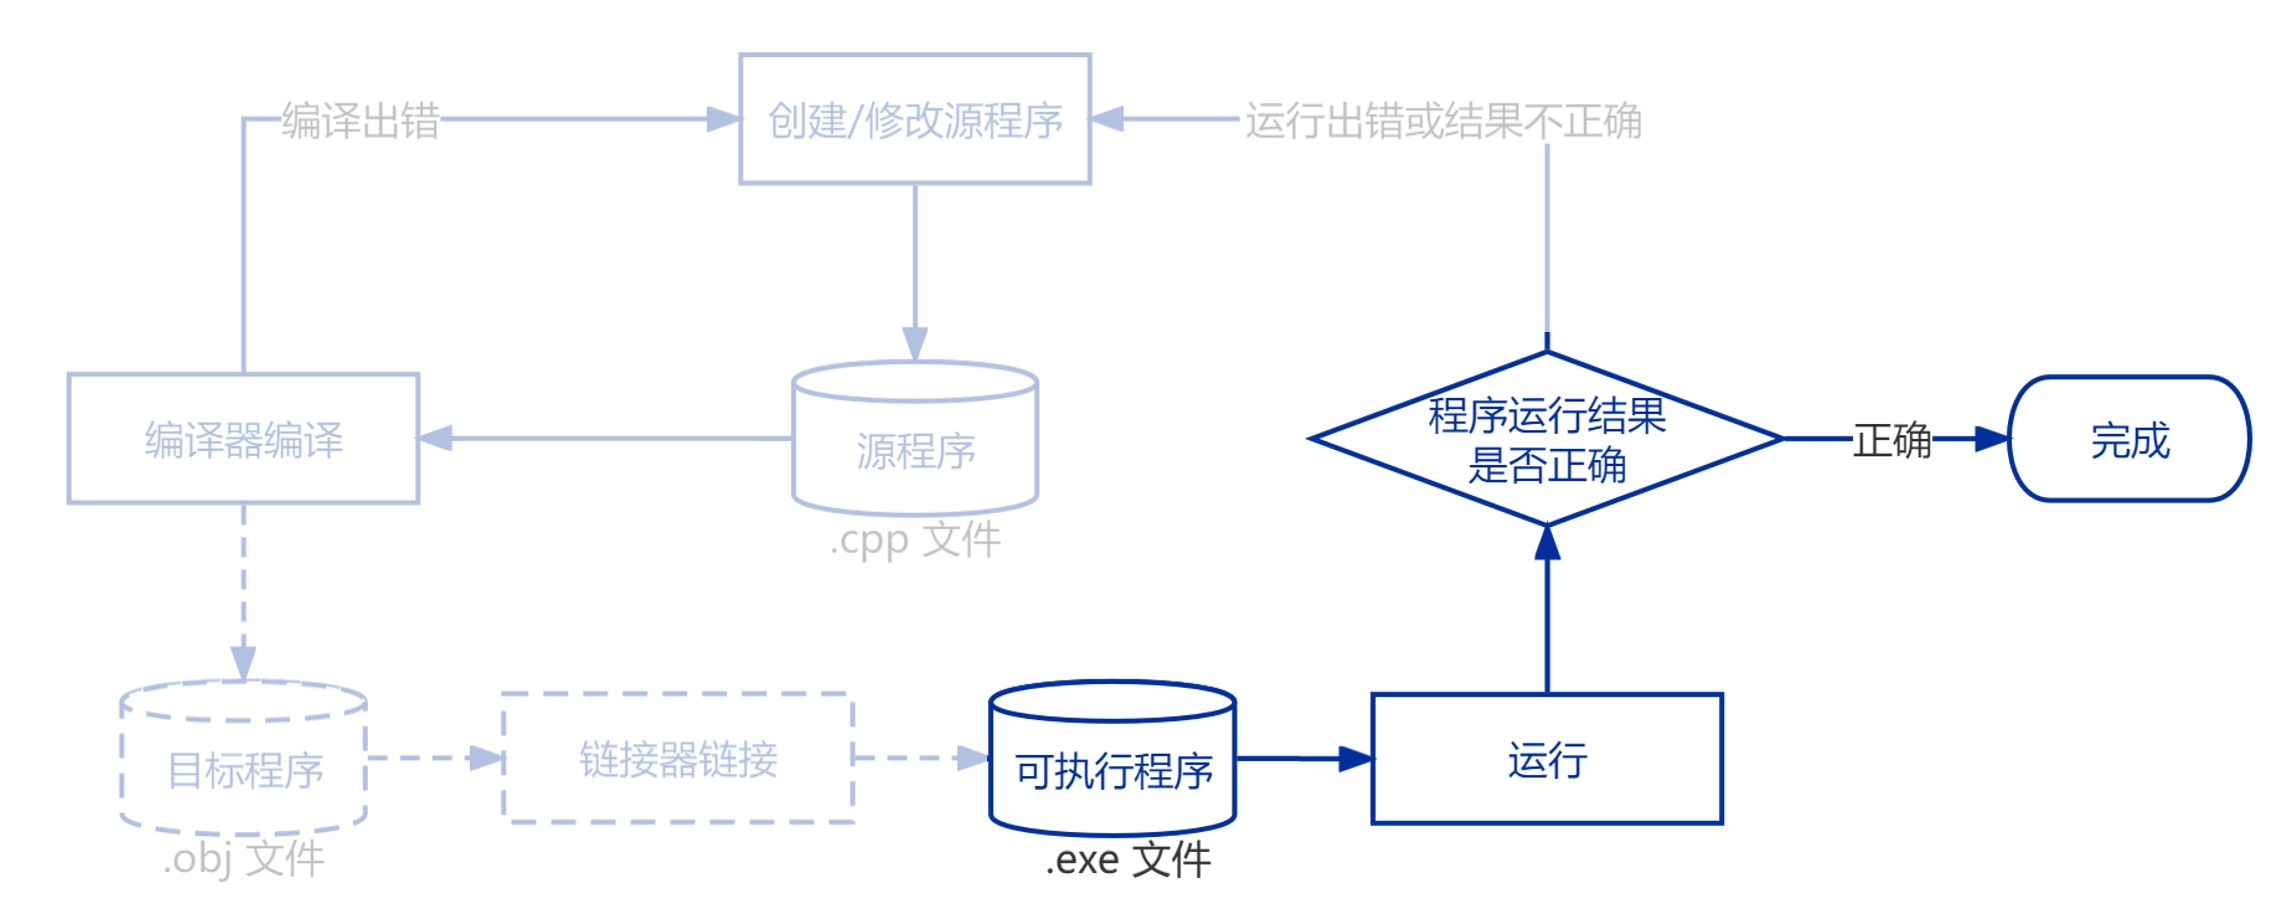
\includegraphics[width=\textwidth]{ch01/run.png}}
    \end{figure}
\end{frame}
%------------------------------------------------------------

%------------------------------------------------------------
\begin{frame}[fragile]
    \frametitle{程序的基本结构}

    \alt<2> {
        \lstinputlisting[basicstyle=\ttfamily\scriptsize,language=C++,name=structure2]{ch01/structure2.cc}
    }{
        \lstinputlisting[basicstyle=\ttfamily\scriptsize,language=C++,name=structure1]{ch01/structure1.cc}
    }
\end{frame}
%------------------------------------------------------------


\section{输出语句}

%------------------------------------------------------------
\begin{frame}[fragile]
    \frametitle{输出语句}

    \begin{itemize}
        \item<1-> 使用 \lstinline|cout| 语句,输出特定内容

        \item<2-> 输出文本

            \begin{itemize}
                \item 文本需要置于双引号 \lstinline|""| 中
                \item \lstinline|cout << "Hello"; // 输出文本信息 Hello| 
            \end{itemize}

        \item<3-> 输出多组文本

            \begin{itemize}
                \item \lstinline|cout << "Hello" << "C++";        // 输出 HelloC++| 
                \item \lstinline|cout << "Hello" << " " << "C++"; // 输出 Hello C++|
                \item 注意,空格也是文本
            \end{itemize}

    \end{itemize}
\end{frame}
%------------------------------------------------------------

%------------------------------------------------------------
\begin{frame}[fragile]
    \frametitle{输出数值}

    \begin{itemize}
        \item<1-> 输出数值

            \begin{itemize}
                \item \lstinline|cout << 100; // 输出数值 100,不需要双引号| 
            \end{itemize}

        \item<2-> 输出多个数值

            \begin{itemize}
                \item
                    \lstinline|cout << 100 << 200;        // 输出 100200| 
                \item
                    \lstinline|cout << 100 << " " << 200; // 输出 100 200| 
            \end{itemize}

    \end{itemize}
\end{frame}
%------------------------------------------------------------

%------------------------------------------------------------
\begin{frame}[fragile]
    \frametitle{如何实现输出两行的效果?}

    \begin{itemize}
        \item 下面的代码可以分开两行输出 \lstinline|Hello World| 吗?

        \item
            \lstinline|cout << "Hello";|\\ 
            \lstinline|cout << "World";|
    \end{itemize}
\end{frame}
%------------------------------------------------------------

%------------------------------------------------------------
\begin{frame}[fragile]
    \frametitle{换行符}

    \begin{itemize}
        \item<1-> C++ 的换行符是 \lstinline|endl|

            \begin{itemize}
                \item 用法:\lstinline|cout << endl;|
                \item 输出一个换行符,使后面的输出从下一行开始
            \end{itemize}

        \item<2->
            \alt<2> {
                \lstinline|cout << "Hello";|\\ 
                \lstinline|cout << "World";|
            }{
                \redout{{\lstinline|cout << "Hello";|}}\\ 
                \redout{{\lstinline|cout << "World";|}}
            }

        \item<3->
            \lstinline|cout << "Hello" << endl;|\\ 
            \lstinline|cout << "World" << endl;|

        \item<4-> 注意,即便输出结果只有一行,一般也要以换行符结尾
    \end{itemize}
\end{frame}
%------------------------------------------------------------

%------------------------------------------------------------
\begin{frame}[fragile]
    \frametitle{格式控制}

    \lstinputlisting[basicstyle=\ttfamily\scriptsize,language=C++,name=format1]{ch01/format1.cc}

    \begin{itemize}
        \item<2-> 输出结果中有几位小数?
        \item<2-> 假如想要保留 $2$ 位小数呢?
    \end{itemize}
\end{frame}
%------------------------------------------------------------

%------------------------------------------------------------
\begin{frame}[fragile]
    \frametitle{保留小数}

    \begin{itemize}[<+->]
        \item 添加头文件 \lstinline|#include <iomanip>|
        \item \lstinline|cout << fixed << setprecision(2) << X.XXX << endl;|
        \item 四舍五入保留 2 位小数
    \end{itemize}
\end{frame}
%------------------------------------------------------------

%------------------------------------------------------------
\begin{frame}[fragile]
    \frametitle{格式控制}

    \lstinputlisting[basicstyle=\ttfamily\scriptsize,language=C++,name=format2]{ch01/format2.cc}

    \begin{itemize}
        \item<2-> 输出结果:3.14
    \end{itemize}
\end{frame}
%------------------------------------------------------------

%------------------------------------------------------------
\begin{frame}[fragile]
    \frametitle{格式控制}

    \lstinputlisting[basicstyle=\ttfamily\scriptsize,language=C++,name=format3]{ch01/format3.cc}

    \begin{itemize}
        \item<2-> 输出结果:3.1416
    \end{itemize}
\end{frame}
%------------------------------------------------------------


\section{总结}

%------------------------------------------------------------
\begin{frame}[fragile]
    \frametitle{总结}

    \begin{itemize}
        \item 计算机的工作原理
        \item 程序语言的发展
        \item C++ 的编译运行
        \item 输出语句
    \end{itemize}
\end{frame}
%------------------------------------------------------------

%------------------------------------------------------------
\begin{frame}
    \begin{center}
        {\Huge Thank you!}
    \end{center}
\end{frame}
%------------------------------------------------------------

\end{document}
